\chapter{Towards measuring Tan's contact in 1D gases}

\section{Tan's contact}

\subsection{Definition from the large momentum tails}

To understand what Tan's contact is, we consider two atoms with contact interactions in the ultracold regime in 1D. The two-body wave-function then only depends from the inter-particle distance $r$ and the scattering length $a_s$ \cite{viverit2004momentum}:

\begin{equation}
    \psi(r) = - \frac{r}{a_s} \, e^{-r/a_s}
\end{equation}

\noindent The Fourier transform of this expression is rather easy to compute and writes:

\begin{equation}
    \tilde{\psi}(k) = \int_0^\infty \psi(r) \, e^{2 \pi i k r} \, dr \propto \frac{1}{(i 2 \pi k - 1/a_s)^2}
\end{equation}

\noindent from which we obtain the momentum distribution:

\begin{equation}
     n(k) = |\tilde{\psi}(k) |^2 \propto \frac{1}{2(2 \pi k a_s)^4 - 2(2 \pi k a_s)^2 +1}
\end{equation}

\noindent Interestingly, if we look at the asymptotic behavior at high $k$ we find that:

\begin{equation}
    n(k) \underrel{k \to \infty} \to \frac{1}{k^4}
    \label{eq:kmf_scaling}
\end{equation}

\noindent Importantly, this signature of contact interactions in the momentum distribution holds for higher dimensions, independently of temperature, interaction strength or quantum statistics making it a \textbf{universal relation}. From equation \ref{eq:kmf_scaling}, we define the Tan's Contact $C$ as:

\begin{equation}
    C = \lim_{k \to \infty} k^4 n(k)
\end{equation}

\subsection{Connection to thermodynamic quantities}

While the $\kmf$ scaling is universal, the value of $C$ depends on the physical characteristics of the system such as the number of particles, temperature, dimension etc. and thus contain meaningful information that would otherwise be hard to measure with standard experimental techniques. This was first theorized by Shina Tan in 2008 \cite{tan2008large} who showed that $C$ is a thermodynamic quantity revealing how the total energy of a two component Fermi gas changes when adiabatically tuning the inverse scattering length $a_s$:

\begin{equation}
    -\frac{d E}{d(1 / a_s)}=\frac{h^{2} C}{2 \pi m}
\end{equation}

\noindent This result is known as Tan's adiabatic sweep theorem and can be adapted to the 1D bosonic case \cite{barth2011tan} to obtain:

\begin{equation}
    C=\left.\frac{4 m}{\hbar^{2}} \frac{\partial \Omega}{\partial a_{1 D}}\right|_{T, \mu}
\end{equation}

\noindent with $\Omega$ the grand potential. This result can also be rewritten to include the interaction energy of the system $\mean{H_{\rm{int}}}$ that we have encountered quite a lot throughout this thesis and is usually hard to measure separately from the total energy:

\begin{equation}
    C=\frac{2 g m^{2}}{\hbar^{4}}\left\langle H_{\text {int }}\right\rangle
    \label{eq:C_with_int}
\end{equation}

\subsection{Characterization of 1D Lieb-Liniger regimes}

Another significant motivation to measure Tan's contact is to characterize the different regimes of Lieb-Liniger 1D systems of interacting bosons as a function of temperature and the strength of the interactions. Tan's contact is indeed particularly suited to study The Lieb-Liniger model as it revolves around the approximation that the interactions between the atoms are repulsive, contact interactions:

\begin{equation}
    H = \sum_j \left[ - \frac{ \hbar^2}{2m} \frac{\partial^2}{\partial^2 {x_j}^2} + V(x_j) \right] + g \sum_{j<l} \delta(x_j - x_l) 
\end{equation}

\noindent with $g$ the strength of the interactions as we have seen on a few occasions in this thesis and $V$ an external trapping potential. 


These different regimes have been widely investigated \cite{petrov2000regimes} and are illustrated on the state diagram of Fig.\ref{fig:1D_diagram}. The lower right part of the diagram corresponds to the strongly interacting or Tonks-Girardeau regime where the repulsive interactions are so strong that they mimic the Pauli exclusion principle for fermions, the gas is then said to fermionize. As the strength of the interactions decreases, the gas progressively goes to a weakly-interacting quasi-condensate phase characterized by suppressed density fluctuations but fluctuating phase, contrary to the true condensate. The nearly ideal gas region refers to the region where the effect of interactions are negligible compared to temperature. \NOTE{voir definitions gamma et t}.

The main difficulty to experimentally characterize those regimes resides in the fact that most quantities show a smooth and monotonic behavior when crossing the transition points between the different regimes. This motivated theoretical studies of the dependency of the Tan's contact with the strength of interactions and temperature to determine whether $C$ constitutes a good probe or not. Previous works have conducted such studies for homogeneous bosons at finite temperature \cite{kheruntsyan2003pair,kormos2009expectation}, trapped bosons at zero temperature \cite{minguzzi2002high,olshanii2003short} or for the trapped finite temperature Tonks-Girardeau regime \cite{vignolo2013universal}. These works were recently completed by \cite{yao2018tan}, characterizing trapped Lieb-Liniger bosons for arbitrary values of the temperature and the interaction parameter.

One of the main experimental difficulties for measuring Tan's contact comes from the fact that the high momentum $\kmf$ tails correspond to very low density values that are hard to detect with classic optical imaging techniques. This problem is however solved with the $\He$ detector thanks to his large dynamic momentum range. Interestingly, our experimental apparatus can be adapted to study 1D physics by transforming our 3D optical lattice into a 2D one as we will see in \ref{sec:1D_exp}, making it the perfect candidate to verify the predictions of \cite{yao2018tan}.

\begin{figure}
    \centering
    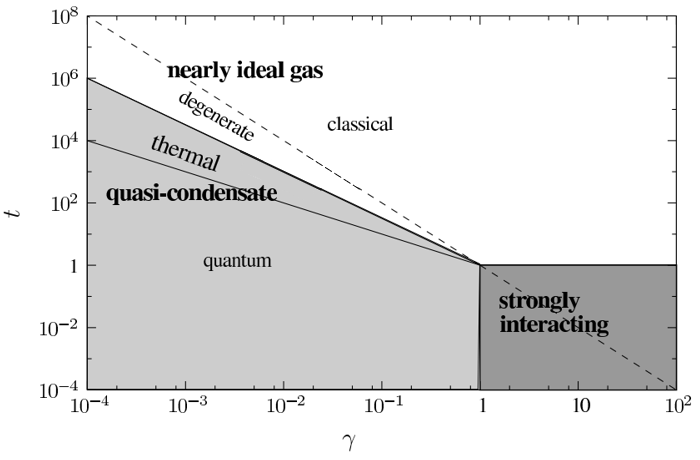
\includegraphics[width=0.8\textwidth]{Fig/Chapter5/quant_degeneracy_1D_trapped.PNG}
    \caption{State diagram of trapped 1D Bose gases with repulsive interactions as a function of the reduced temperature $t$ and the interaction parameter $\gamma$. The dashed diagonal line separates the classical and quantum degenerate regimes, while the solid lines indicate smooth crossovers between the different regimes.}
    \label{fig:1D_diagram}
\end{figure}


\section{Theoretical study}

\label{sec:1D_theory}

Before going into the experimental details, we start our study by summarizing the main results of \cite{yao2018tan}.

\subsection{Two-parameter scaling}

At first glance, Tan's contact should depend from 4 parameters:

\begin{itemize}
    \item The total number of particles $N$.
    \item The temperature $T$.
    \item The trapping frequency $\omega_{\rm{1D}}$.
    \item The coupling constant $g$.
\end{itemize}

\noindent The first result of \cite{yao2018tan} is to show that $C$ actually depends from only two parameters, the first one being the reduced interaction strength:

\begin{equation}
    \xi_{\gamma}=-a_{\rm{ho}}/a_{\rm{1D}}\sqrt{N}
\end{equation}

\noindent with $a_{\rm{ho}}=\sqrt{\hbar/m \omega_{\rm{1D}}}$ the harmonic oscillator length and $a_{\rm{1D}}=a_{\rm{oh}}^2/a_s$ the 1D scattering length. The second one is the reduced temperature

\begin{equation}
    \xi_T=-a_{\rm{1D}}/\lambda_T
\end{equation}

\noindent with $\lambda_T=\sqrt{2\pi \hbar^2/m k_b T}$. The contact can then be written as a function of $\xi_{\gamma}$ and $\xi_{T}$:

\begin{equation}
    C= \frac{N^{5/2}}{a_{\rm{ho}}^3} f(\xi_{\gamma},\xi_{T})
\end{equation}

The goal is then to determine the variations of $f(\xi_{\gamma},\xi_{T})$. To do so, the authors of \cite{yao2018tan} follow two complementary approach. The first one consists in using the Bethe Ansatz which is the exact solution of the Yang-Yang equations \cite{yang1969thermodynamics} of the 1D homogeneous gas. The results are adapted to the trapped case by using the Local Density Approximation (LDA) as we did in \ref{sec:ch2_trapping_effects}. The validity of this approach is checked by comparing its prediction to {\it ab-initio} QCM calculations as shown on Fig-\ref{fig:C_theo}.

\begin{figure}
    \centering
    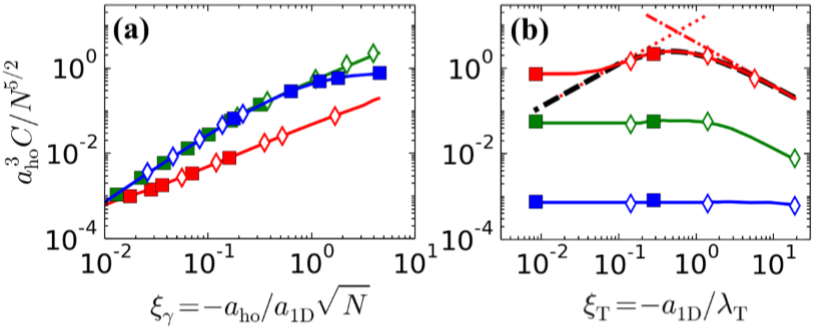
\includegraphics[width=0.9\textwidth]{Fig/Chapter5/BS_LDA_vs_Bethe.PNG}
    \caption{Reduced contact $a_{ho}^3 C_3 / N^{5/2}$ as a function of $\xi_T$ and $\xi_{\gamma}$ as predicted from the LDA approach (solid lines) and QMC calculations (points). The different symbols correspond to various parameters for the QMC calculations (see \cite{yao2018tan} for further details). (a) Reduced contact versus $\xi_{\gamma}$ at fixed temperatures corresponding to $\xi_T = 0.0085$ (blue), 0.28 (green), and 18.8 (red). (b) (b) Reduced contact versus $\xi_T$  at fixed interaction strengths corresponding to $\xi_\gamma = 10^{-2}$ (blue), $1.58 \times 10^{-1}$ (green), and 4.47 (red). The black dashed, red dotted, and red dash-dotted lines correspond to \NOTE{todo} respectively. }
    \label{fig:C_theo}
\end{figure}

\subsection{Maximum contact versus temperature}

A striking and unexpected feature of Fig.-\ref{fig:C_theo} panel (b) is that the contact shows a non-monotonous dependency with $\xi_T$ with a maximum, contrary to the monotonous increase in the Tonks-Girardeau regime predicted by \cite{vignolo2013universal}. While the maximum exists for any value of $\xi_{\gamma}$, the effect is more pronounced in the strongly-interacting regime. 

\subsubsection{Strongly-interacting regime}

In this regime, the contact can be determined analytically via a virial expansion \cite{vignolo2013universal} and writes:

\begin{equation}
    C = \frac{2 N^{5/2}}{\pi a_{ho}^3} \frac{\xi_\gamma}{\xi_T} \left( \sqrt{2} - \frac{e^{1/2 \pi \xi_T^2}}{\xi_T} \textrm{Erfc}(1/\sqrt{2 \pi} \xi_T) \right)
    \label{eq:C_strong_int}
\end{equation}

In the asymptotic regime of low-temperature limit $\xi_\gamma^{-1} \leq \xi_T \leq 1$, this expression simplifies to:

\begin{equation}
    C = 2 \sqrt{2} \, \frac{N^{5/2}}{a_{ho}^3} \, \xi_\gamma \, \xi_T 
    \label{eq:strong_int_lowT}
\end{equation}

\noindent In the opposite regime of high-temperature $\xi_\gamma^{-1}, \, 1 \leq \sqrt{\xi_T}$, we rather get:

\begin{equation}
    C \simeq 2 \sqrt{2} \, \frac{N^{5/2}}{ \pi a_{ho}^3} \, \frac{\xi_\gamma}{\xi_T} 
    \label{eq:BS_strong_int_highT}
\end{equation}

\noindent We thus clearly see the non-monotonic behavior of the contact. These 3 expressions are plotted in dashed line on Fig-\ref{fig:C_theo}. We see that the full analytical expression of \ref{eq:C_strong_int} (black dashed line) well matches the LDA predictions, except for low-temperatures for which the virial expansion is not suited.

The existence of a maximum value of the contact can be understood by the competition between the effect of temperature and interactions. While interaction dominates, the gas is fermionized and the contact increases with temperature \cite{vignolo2013universal}, whereas it decreases as thermal fluctuations take over and fermionization disappears. The location of the maximum of the contact thus provides a way to characterize the crossover to fermionization. 

\subsubsection{Weakly-interacting regime}

In the weakly-interacting regime, the interactions are not strong enough to fermionize the gas. In the low-temperature regime $1, \, \xi_T \leq \xi_\gamma^{-1}$, the gas forms a quasi-condensate and the contact is obtained from equation \ref{eq:C_with_int} with the mean-field expression of $H_{\text {int }}$ and writes:

\begin{equation}
    C = \eta \frac{N^{5/2}}{a_{ho}^3} \xi_\gamma^{5/3} 
    \label{eq:weak_int_lowT}
\end{equation}

\noindent with $\eta = 4 \times 3^{2/3}/5$. We see that $C$ does not depend from temperature here. At high temperatures $\xi_\gamma^{-1} \leq \xi_T \leq \xi_\gamma^{-2}$, interactions become negligible so that the gas is nearly ideal and the contact writes:

\begin{equation}
    C = \left( 16 \sqrt{\pi} \, \frac{N^{5/2}}{a_{ho}^3} \, \xi_\gamma^5 \, \xi_T^3 \right) G(\alpha) \, ,
    \label{eq:weak_int_highT}
\end{equation}

\noindent with $G(\alpha)$ decreasing at least in $\lambda_T^4$ (see \cite{yao2018tan} for the explicit expression), making $C$ decrease with temperature. Once again, identifying the temperature at which $C$ starts to decay allows to characterize the crossover between the quasi-condensate regime and the nearly ideal Bose gas regime.

\section{Experimental realisation of 1D gases with the optical lattice}

\label{sec:1D_exp}

Now that we have seen what Tan's contact is and how it could be used to characterize the regimes of Lieb-Liniger 1D gases, we will show how our experimental apparatus can be adapted to study 1D physics with the objective of testing experimentally the predictions of \cite{yao2018tan}. The main idea to obtain an  experimental 1D system is to ``freeze'' the degrees of freedom of the atoms in two directions of space. To do so, the easiest solution is to use a harmonic trapping potential with trapping frequencies $\omega_{\perp}$ high enough so that the energy difference $\Delta E =\hbar \omega_{\perp}$ between the ground-state and the first excited state is much larger than the typical energy of the atoms $\Delta E \gg \kB T, \mu$. Such high trapping frequencies are accessible in our experiment thanks to the optical lattice. Instead of using the 3 pairs of countra-propagating beam as we did so far, we use only 2 to produce a 2D lattice. Interestingly, the total laser power is divided amongst 2 pair of beams instead of 3, meaning that we can reach much higher values of the lattice depth, typically up to $s=30$. In the direction where there is no lattice, the trapping potential results from the Gaussian shape of the beams and has a trapping frequency $\omega_{\rm{1D}} =2 \pi \times 140 \sqrt{s} = 2 \pi  \times 713 \ \rm{Hz}$ for $s=26$. In the other 2 directions, the trapping frequency is however very large as a result of the lattice interference pattern $\omega_{\perp} \simeq 200 \ \rm{kHz}$, which is much larger than the energy of the atoms $\kB T, \mu \simeq 25 \ \rm{kHz}$ with typical experimental parameters.

\begin{figure}
    \centering
    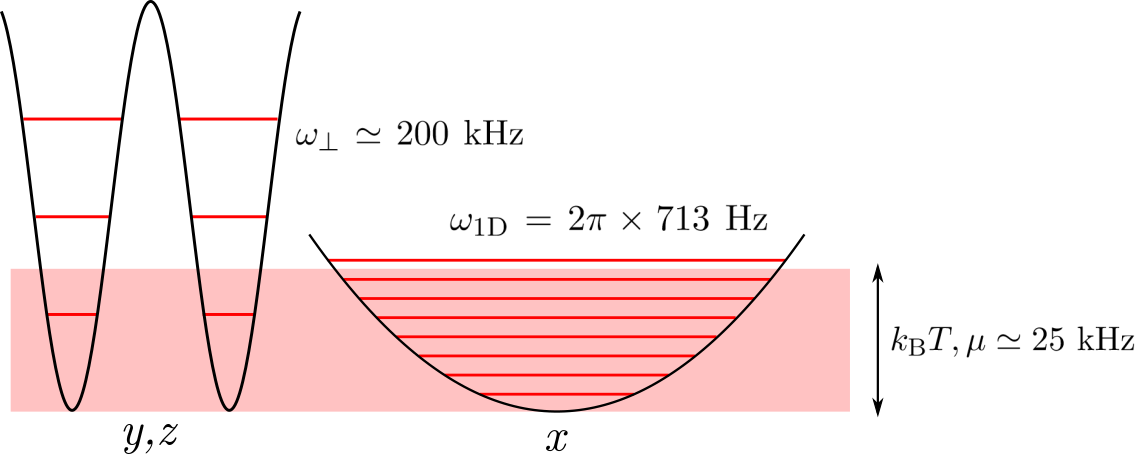
\includegraphics[width=0.9\textwidth]{Fig/Chapter5/1D_config.png}
    \caption{Configuration of the optical lattice to produce 1D tubes. In the transverse direction, the lattice interference pattern creates a confining potential that can be approximated to a harmonic potential near the center of the site. The trapping frequency is high enough so that the degree of freedom of the atoms in these directions is ``frozen''. On the other hand, the lattice is absent in the longitudinal direction and the trapping frequency only results from the Gaussian shape of the beams. This is the 1D direction.}
    \label{fig:my_label}
\end{figure}


Using the optical lattice in this configuration then allows us to emulated 1D physics. The main drawback of this method is that we end up with an array of 1D gases rather than a single one, complicating the comparison with theory.


\subsection{Characterization of the 1D tubes}

\subsubsection{Number of atoms}

The major difficulty comes from the fact the atom number varies from one 1D tube to another. To determine the atom number distribution, we first need to determine the density profile of the cloud in the 2D lattice.

To do so, we first remind that under the Thomas-Fermi approximation (\NOTE{ref}), the density profile of a BEC in a 3D harmonic potential writes:

\begin{equation}
     n(\bm{r}) = \frac{\mu}{g} \, \left[ 1 - \left( \frac{x}{R_x} \right)^2 - \left( \frac{y}{R_y} \right)^2 - \left( \frac{z}{R_z} \right)^2 \right]
\end{equation}

\noindent where $R_i = \sqrt{\frac{2 \mu}{m \omega_i^2}}$ is the Thomas-Fermi radius in direction $i$. Under the mean-field approximation, the chemical potential is:

\begin{equation}
     \mu = \frac{\hbar \bar{\omega}}{2} \left(  15 N_{\rm{tot}} \frac{a_s}{a_{\rm{ho}}}\right)^{2/5}
\end{equation}

\noindent with $\bar{\omega}=\omega_x \omega_y \omega_z/3$ the average trapping frequency.

Similarly to the method developed in \ref{sec:rescaled_interaction}, we rescale $\mu$ to account for the presence of the 2D lattice with:

\begin{equation}
    \tilde{\mu} = \frac{\hbar \bar{\omega}}{2} \left(  15 N_{\rm{tot}} \frac{\tilde{a}_s}{a_{\rm{ho}}}\right)^{2/5}
\end{equation}

\noindent where $\tilde{a}_s= a_s \left(d \int_0^d |u_{0,0} (x)|^4 \mathrm{d}x \right)^2$ is the rescaled interaction strength, with the notable difference that we are using here a power 2 instead of power 3 in \ref{sec:rescaled_interaction} as we use here a 2D lattice. \NOTE{vérifier} We finally obtain the new Thomas-Fermi radius in the transverse directions

\begin{equation}
    R_{\rm{TF}} = \frac{1}{d} \sqrt{\frac{2 \tilde{\mu}}{m \omega_{\perp}^2}}
\end{equation}

\noindent that we express in units of lattice spacing $d$ for convenience. The number of atoms in the tube indexed $j,l$ then writes:

\begin{equation}\label{eq:N_per_tube}
    N_{j,l} = N_{00} \left( 1 - \frac{j^2 + l^2}{R_{\rm{TF}}^2} \right) .
\end{equation}

\noindent where $N_{00}$ is the number of atoms in the central tube. We deduce $N_{00}$ from the total atom number $\NBEC$ with the normalization condition $\NBEC = \sum_{j,l} N_{j,l}$ giving:

\begin{equation}
    N_{00} = \frac{5}{2 \pi} \frac{\NBEC}{R_{\rm{TF}^2}}
\end{equation}

\begin{figure}
    \centering
    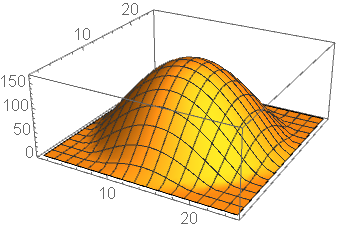
\includegraphics[width=0.6\textwidth]{Fig/Chapter5/atomic_distrib_2Dlatt.PNG}
    \caption{Atom number distribution in a 2D lattice of amplitude $s=26$ for $\NBEC=30 \times 10^3$.}
    \label{fig:my_label}
\end{figure}

\begin{figure}
    \centering
    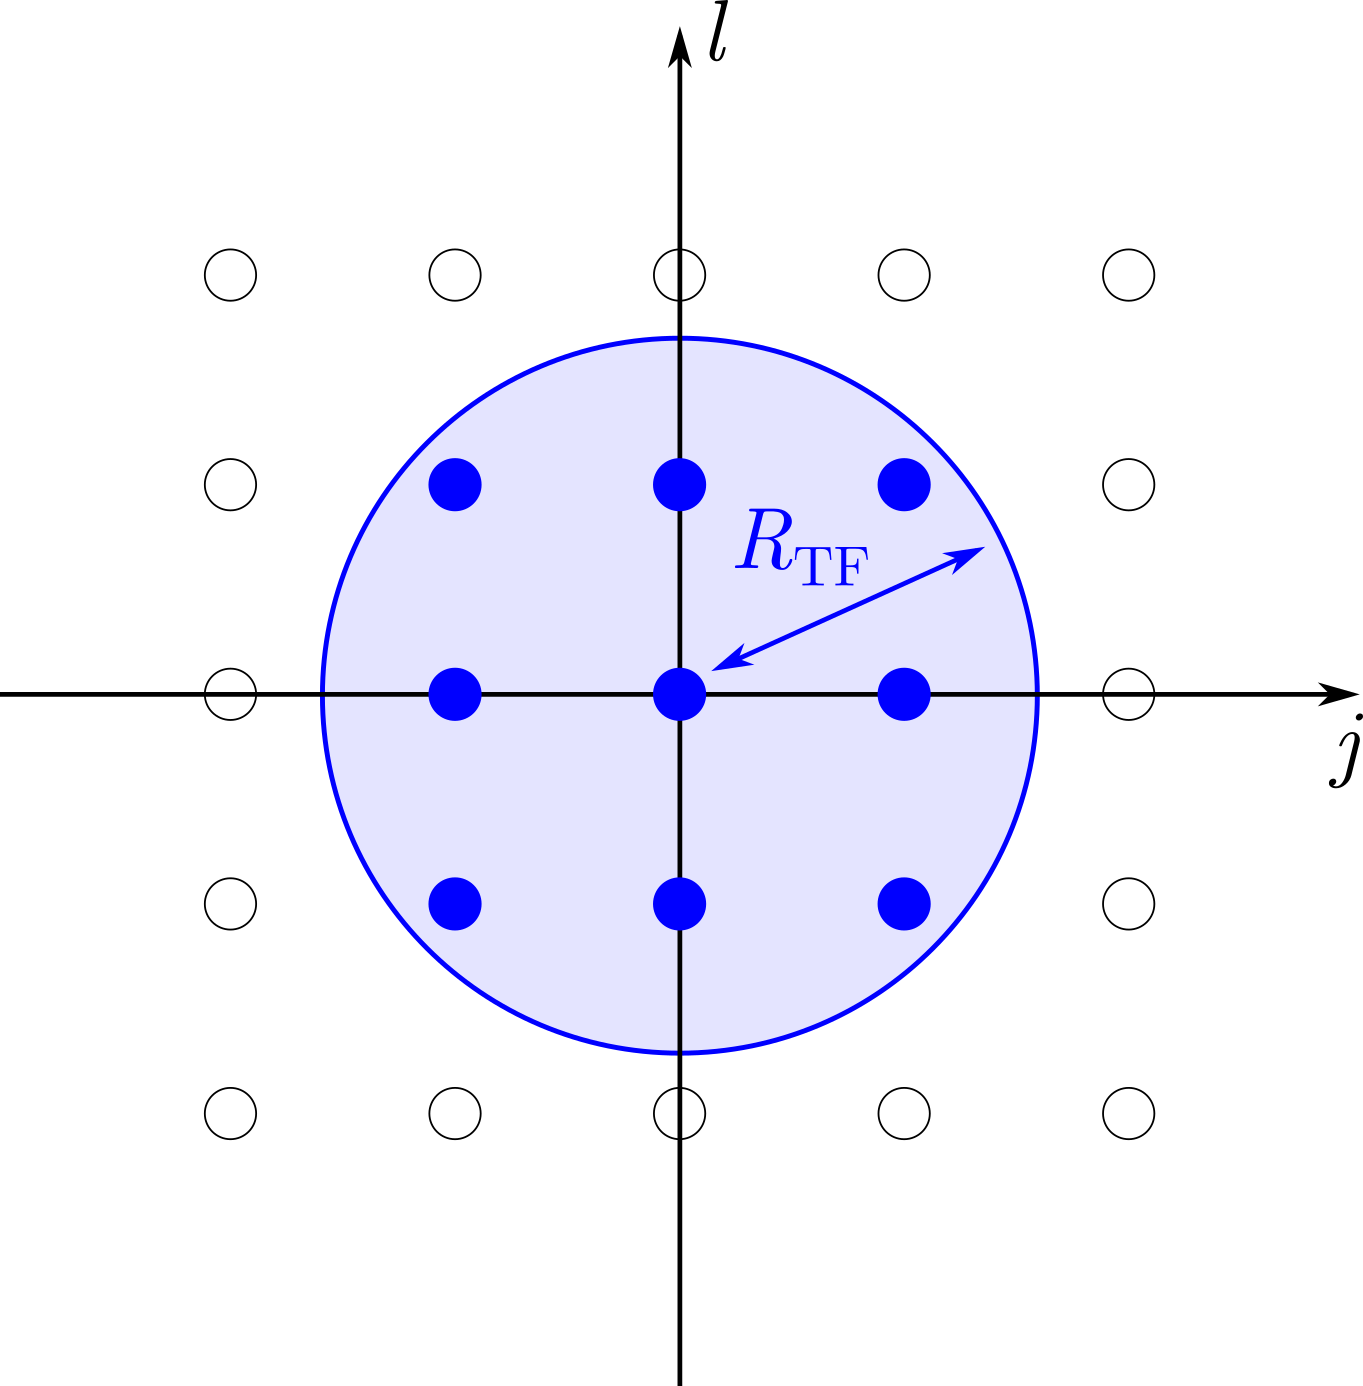
\includegraphics[width=0.45\textwidth]{Fig/Chapter5/tubes_occupes.png}
    \caption{Schematic of the array of 1D tubes. The large blue circle denotes the parabolic density profile of the BEC that determines which of the lattice sites contain atoms (blue dots).}
    \label{fig:my_label}
\end{figure}

\subsubsection{Density and interaction parameter}

Knowing the number of atom in each tube, we now look to determine the density and interaction parameter $\gamma$ in each of the tubes. To do so, we first introduce the effective 1D interaction strength $g_{\rm{1D}} \simeq 2 \hbar \omega_{\perp} a_s$ \cite{olshanii1998atomic} that depends from the transverse trapping frequency and the 3D scattering length. With this definition, we can write the 1D chemical potential and 1D density for the different tubes, both functions of the number of atoms in the tube:

\begin{equation}
    \mu_{1D}^{j,l} = \left( \frac{3}{4 \sqrt{2}} \, N_{j,l}\,  g_{1D} \, \omega_{1D}\,  \sqrt{m} \right)^{2/3}
\end{equation}

\begin{equation}\label{eq:n_1D}
    \rho_{1D}^{j,l}(x) = \frac{\mu_{1D}}{g_{1D}} - \frac{1}{2} \, m \, \omega_{1D}^2 \, x^2
\end{equation}

\noindent In practice, the second term of equation \ref{eq:n_1D} can be neglected because of the small size of the 1D gases $\sim \mu \rm{m}$ and the weak confinement $\omega_{1D} \approx 2 \pi \times 700 \rm{kHz}$ so that $\rho_{1D}^{j,l}(x)$ is constant and well approximated by its value at the center of the trap $\rho_{1D}^{j,l}(0)$. We then simply write $\rho_{1D}^{j,l}$.

Finally, we can write the interaction parameter $\gamma$ corresponding to the ratio between the interaction and the kinetic energy:

\begin{equation}
    \gamma_{j,l} = \frac{m \, g_{1D}}{\hbar n^{j,l}_{1D}} 
\end{equation}

\subsubsection{Weighted average}

\noindent The values of $\gamma_{j,l}$ \NOTE{à voir} for each of the 1D tubes are however not very meaningful in practice as the distribution that we measure results from the contribution of every lattice tubes. It is therefore more convenient to define a single averaged value of $\bar{\gamma}$ to approximately describe the entire ensemble of 1D gases. One could first simply think of using a simple average:

\begin{equation}
    \bar{\gamma} = \frac{1}{N_{\rm{tubes}}} \sum_{j,l} \gamma_{j,l}
\end{equation}

\noindent This kind of averaging is however too strong of an approximation as it assumes that each of the tubes contribute equally to the total measured distribution which is wrong as the contribution of the tubes with more atoms will be more significant. We then chose to weight the contribution of each of the tubes in the average by its fraction of the total atom number:

\begin{equation}
    \bar{\gamma} = \sum_{j,l} \frac{N_{j,l}}{\NBEC} \gamma_{j,l}
\end{equation}

\noindent Note that this kind of averaging can be done for all relevant quantities that vary from one 1D tube to another.



\subsection{Independence of the tubes}

In order to properly observe 1D physics, it is crucial that all the 1D tubes are independent from one another, \ie no coherence subsists in the transverse directions. This is true when the typical timescale \NOTE{faire cette section}

\section{Detection of large momentum components}

While the great sensitivity of the $\He$ detector is perfectly suited to detect the very low density $\kmf$ momentum tails, the size of the MCPs limits the range of detector. From the work \cite{xu2015universal}, we obtain that the $\kmf$ decay should start around $k_0 \sim 1.6 \times \rho_{\rm{1D}}(0)$ \NOTE{blah blah chiffres}.

\subsection{Magnetic gradient and displacement procedure}

One solution to this issue is to give the entire cloud a momentum kick in the first instants of the TOF to artificially change the momentum range of the $\He$ detector. With our experimental setup, the easiest way to do so is to create a magnetic gradient to apply a magnetic force on the atoms during a time $t_{\rm{grad}}$ before transferring them to the $m_j=0$ sub-state. 

This technique however brings some experimental complications as the population transfer cannot be done immediately after turning off the trap. As a matter of fact, the atoms starts moving during the time $t_{\rm{grad}}$ and will therefore be at different positions when the transfer is performed. The problem comes from the fact that there is a slight inhomogeneity in the bias field along direction $x$ used to set the energy difference between the sub-states $m_j=0$ and $m_j=1$. This means that the resonance condition for a Raman or RF transfer depends on the initial momentum of the atoms, with the consequence that we cannot properly transfer the whole cloud to $m_j=0$ with a simple single frequency Rabi pulse.

To solve this issue, \NOTE{expliquer rapidement sweep}. We understand however that it is increasingly difficult to fulfill the adiabatic condition for all momentum classes if the spread in resonance frequencies is too high. We therefore need to devise a displacement sequence as short as possible to minimize the distance travelled by the atoms before the transfer, as well as to make sure that the magnetic gradient is properly turned off not to further increase the field inhomogeneity.

The procedure is represented on Fig.-\ref{fig:displacement_sequence}. Right after the lattice is turned off, we increase the current in the MOT coils to produce the magnetic gradient. The MOT coils are indeed the coils with which we can produce the stronger gradient, reducing the time during which we need to apply it to reach the proper momentum shift. However, the current in the MOT coils typically needs around $10 \ \rm{ms}$ to reach the highest possible values, which is already too long. We then set the command voltage $V_{\rm{command}}$ to be close to the highest possible value, let the current increase for $t_1 = 1 \ \rm{ms}$ and then set the command to $0$ and let the current decay for $t_2-t_1=13 \ \rm{ms}$ \NOTE{check numbers} until it is fully turned off. After that, we finally perform the population transfer and let the atoms fall unto the MCP. The momentum displacement of the cloud can be set by changing the command voltage $V_{\rm{command}}$.

\begin{figure}
    \centering
    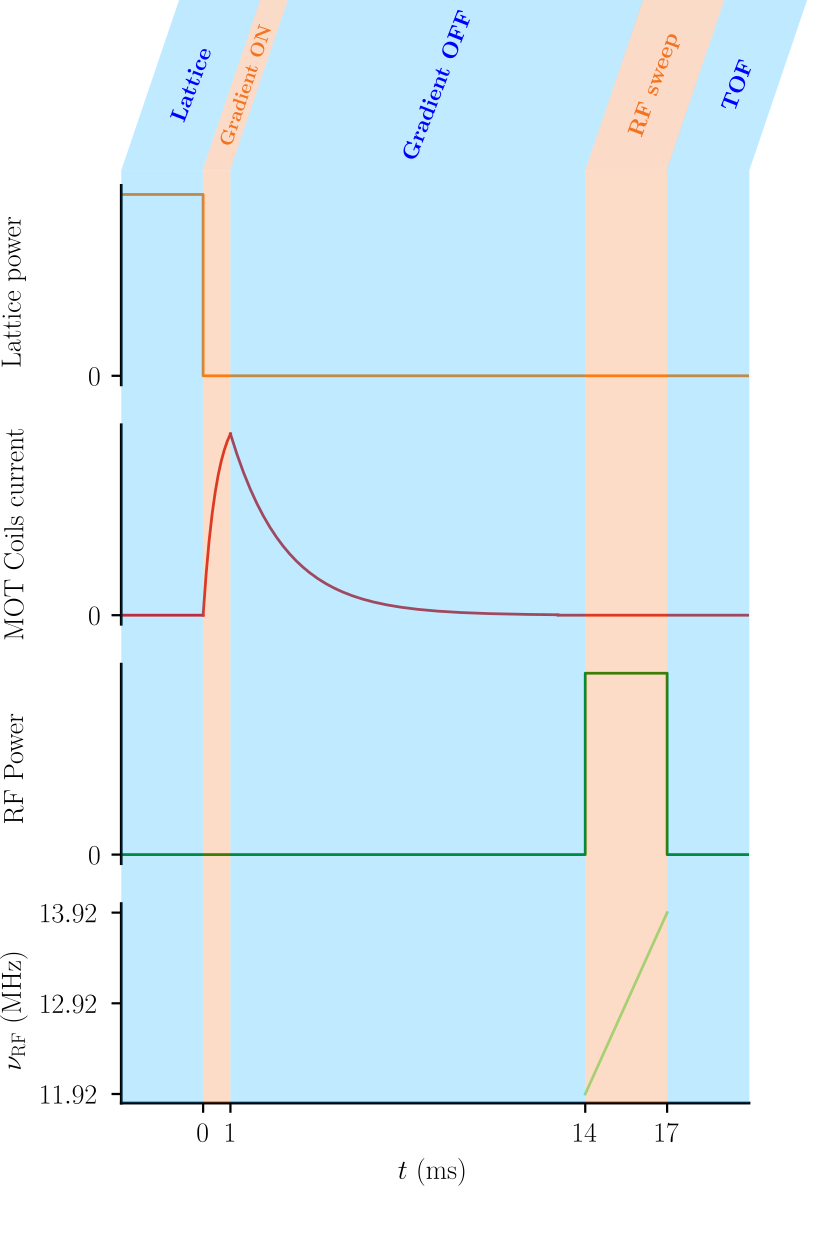
\includegraphics[width=0.8\textwidth]{Fig/Chapter5/displacement_sequence.png}
    \caption{Experimental sequence to shift the entire momentum distribution so that the $\kmf$ tails fall unto the $\He$ detector.}
    \label{fig:displacement_sequence}
\end{figure}

\subsection{Benchmarking with 3D lattice gases momentum distribution}

To test that our method does not induce any distortion of the momentum distribution, we benchmark it with 3D lattice gas momentum distribution slightly above the Mott critical point so that the momentum distribution has a wide background but still sharp diffraction peaks. This allows to check for distortion at high momentum values, while making more precise measurements with the narrow diffraction peaks \NOTE{vraiment pas ouf}.





\section{Experimental study}

\subsection{Analysis of the transverse shape}

The first thing that we need to check is the transverse shape of the 3D distribution to know whether we can fully decouple what is happening in the 1D direction from what is happening in the other two transverse directions. The transverse momentum distribution is supposed to be a Gaussian distribution whose width depends on the transverse trapping frequency. If the atoms are in the harmonic oscillator ground state of the transverse direction, the RMS width of the distribution in momentum space is $\Delta k_{\rm{theo}}=\sqrt{\frac{m \omega_{\perp}}{2 \hbar}}$. \NOTE{factor 2?}
\paragraph{} On Fig.-\ref{fig:1D_transverse}, we plot the transverse distribution along gravity at different positions along the 1D direction and normalize it to 1. We observe that we get the same RMS size for every $k_{\rm{1D}}$ at which the cut is done meaning that the 1D direction is fully decoupled from what is happening in the transverse direction. We extract its RMS width \fcolorbox{red}{white}{$\Delta k_{\rm{exp}}=5.96(2) \mu \rm{m}^{-1}$}. This data set was taken with $s=26$, meaning that $\omega_{\rm{site}}=1.33 \times 10^6$ Hz \NOTE{errorbar?}, giving \fcolorbox{red}{white}{$\Delta k_{\rm{theo}}=6.4 \mu \rm{m}^{-1}$} so a reasonable agreement between the two values. \NOTE{notations}

\begin{figure}
    \centering
    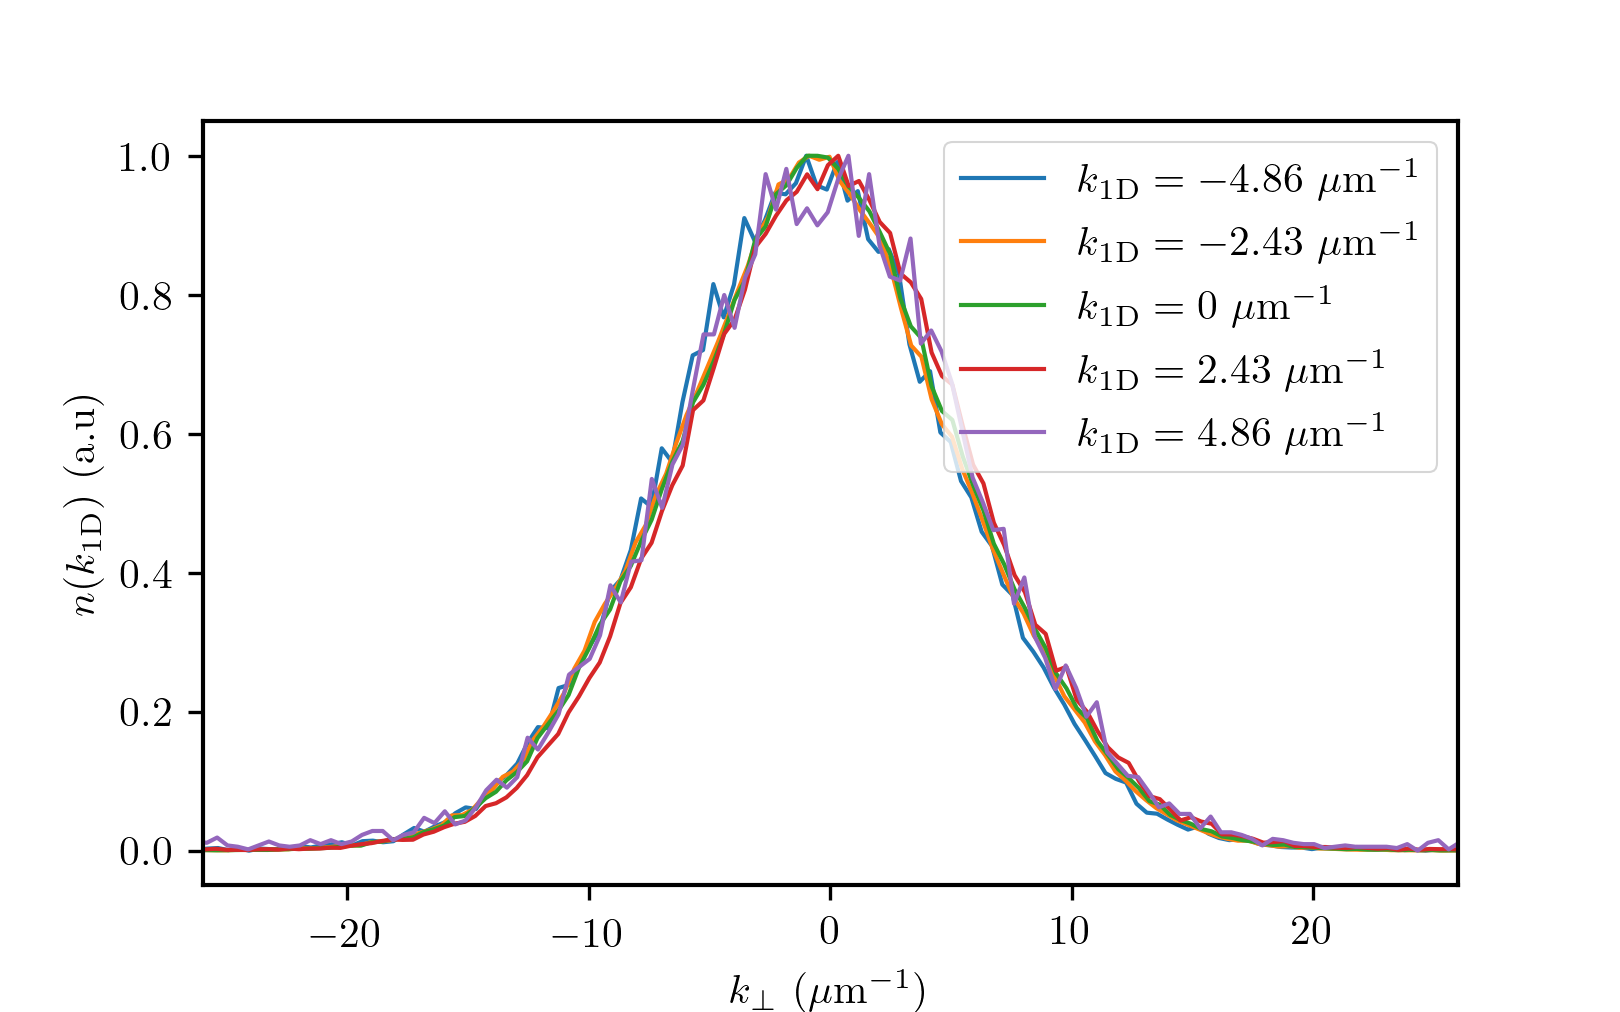
\includegraphics[width=0.9\textwidth]{Fig/Chapter5/1D_transverse_effect.png}
    \caption{Caption}
    \label{fig:1D_transverse}
\end{figure}

\subsection{Calculation of the momentum density}


\label{sec:1D_calculation_momentum_density}

In order to compare the experimental values of the Tan's contact to theory, it is crucial to obtain the absolute value of the 1D density $n_{\rm{1D}}(k)$ from the experimental data. To do so, we exploit the fact that the transverse distribution shape is the same along the 1D direction as we have just seen. Under the effect of the fast transverse expansion, some atoms fall beyond the MCP and are therefore not detected. However, knowing the transverse profile, we can do as if everything was only happening in one direction and integrate over the transverse profile. The procedure is the following:

\begin{itemize}
    \item We plot the transverse distribution (in the vertical direction where it is not cut out by the finite size of the $\He$ detector) and extract its RMS width $\sigma$. \NOTE{notations}
    \item For one pixel of size $\Delta k_{1D} \times \Delta k_{\perp}^2$, we have (keeping in mind normalization condition with the factor $2\pi$) \NOTE{vérifier ça}:
    

    \begin{align}
        n_{1D}(k) &= 2\pi \times \frac{N_{\rm{vox}}(k)}{\eta \Delta k_{1D} \Delta k_{\perp}^2} \left(\int n_{\perp}(k) dk \right)^2 \\
        % &=2\pi \times \frac{N_{\rm{pix}}(k)}{\eta \delta k_{1D} \delta k_{\perp}^2} 2 \pi \sigma 
    \end{align}
    
    \noindent $\eta$ being the detection efficiency and $N_{\rm{pix}}$ the number of atoms in the voxel at a given $k$. From this, we obtain the expression of $n_{\rm{1D}}(k)$ that depends only on known experimental values:
    
    \begin{equation}
        n_{1D}(k) = 4\pi^2 \times \frac{N_{\rm{pix}}(k)}{\eta \delta k_{1D} \delta k_{\perp}^2} \sigma 
    \end{equation}

    

\end{itemize}

\subsection{Transverse integration effects}

As in \ref{sec:transverse_integration}, the transverse size of the voxels defines a transverse integration $\Delta k_{\perp}$ that needs to be sufficiently large \NOTE{number} to ensure a proper signal to noise ratio. As illustrated on Fig.\ref{fig:1D_integration}, the transverse integration however effectively reduces the momentum range in the 1D direction because of the circular shape of the detector that cuts out a part of the integration volume. The transverse integration must then be kept as low as possible and the distorted edges of the distribution ignored in the analysis. 

\begin{figure}
    \centering
    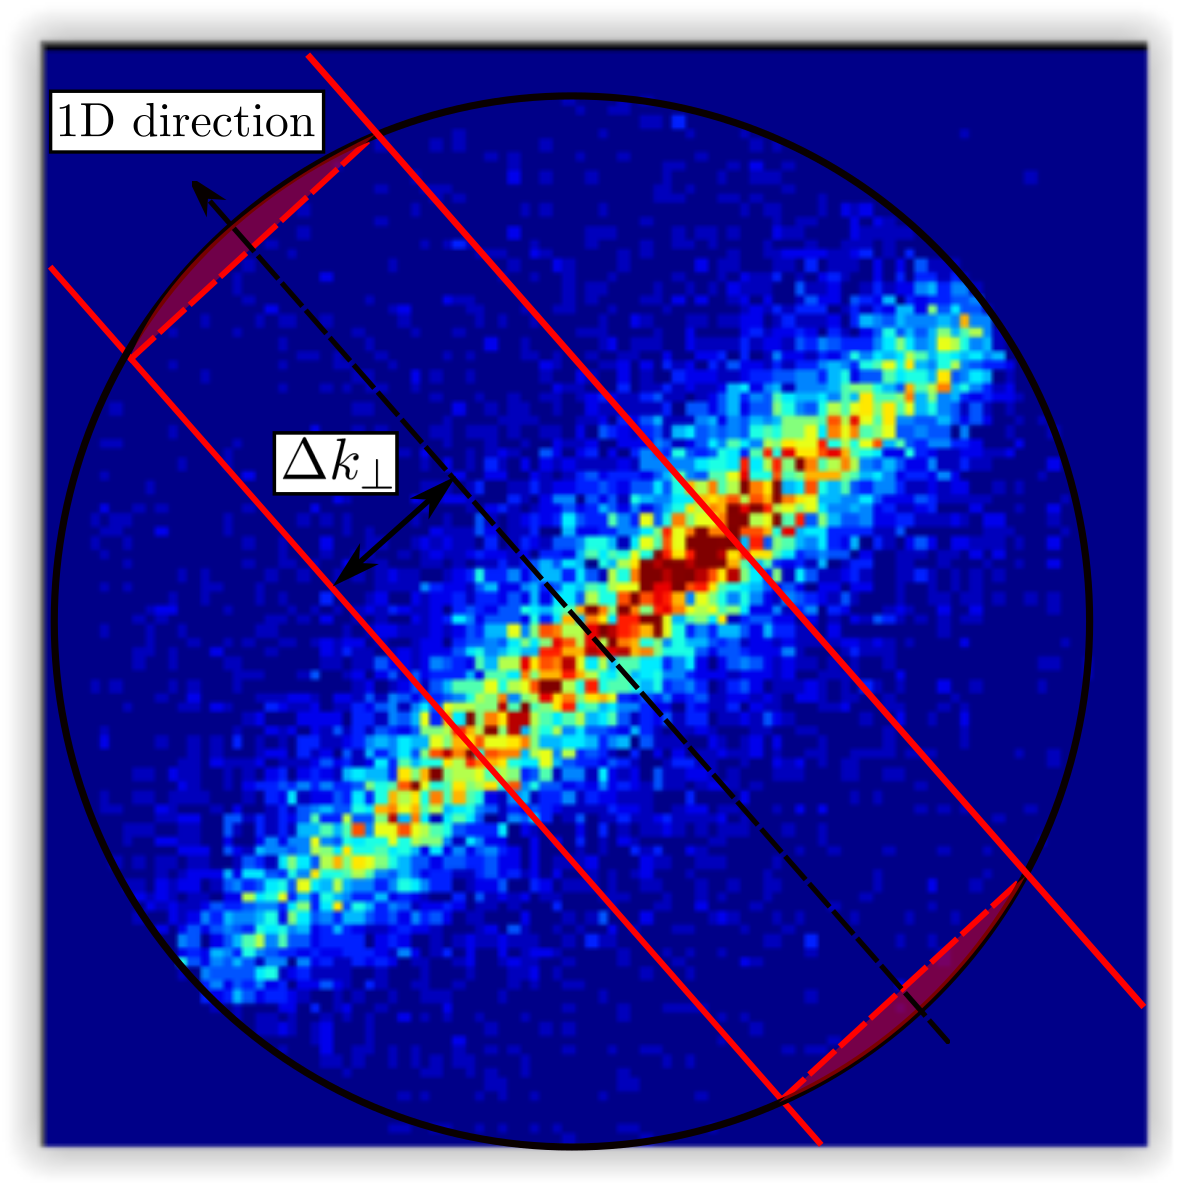
\includegraphics[width=0.7\textwidth]{Fig/Chapter5/1D_transverse_integration.png}
    \caption{Gravity integrated 2D image of the distribution of the 1D lattice gas illustrating the effect of the transverse integration. The red shaded area indicated the region where the geometry of the detector affects the measurement of $n_{\rm{1D}} (k)$.}
    \label{fig:1D_integration}
\end{figure}

\subsection{Measurement of the temperature}

\label{sec:1D_temperature}

As we want to study the dependency of the Tan's contact with temperature as well make comparison with QMC calculations, we first need to extract the temperature from the experimental data. This is easier than for 3D Bose-Hubbard gases as the width of the momentum distribution gives information about the temperature of the gas. At low values of $k$, the shape of the 1D momentum density is Lorentzian as illustrated on Fig.\ref{fig:1D_temperature}. \NOTE{refs} The temperature of the gas can be extracted from the width of the Lorenztian shape using 

\begin{equation}
    n(k)=\frac{2n/\Delta k }{1+(k/\Delta k)^2}
\end{equation}

\noindent with $n$ the maximum density ({\color{blue}[CHECK]}) and:

\begin{equation}
    \Delta k=\frac{m k_b T}{\hbar^2 \rho_{1D}(0)} \alpha_{\rm{fit}}
\end{equation}

\noindent with $\rho_{1D}(0)$ the spatial density at the center of the tube and $\alpha_{\rm{fit}}$ a coefficient to take into account the effect of the trapping potential. This coefficient varies slightly with the interaction parameter $\gamma$ and has been calibrated through QMC calculations. We use a $\rho_{1D}(0)$ which correspond to the weighted averaged $\rho_{1D}(0)$ over the tube distribution. {\color{blue}(good choice of $\rho_{1D}(0)$)?}.

\begin{figure}
    \centering
    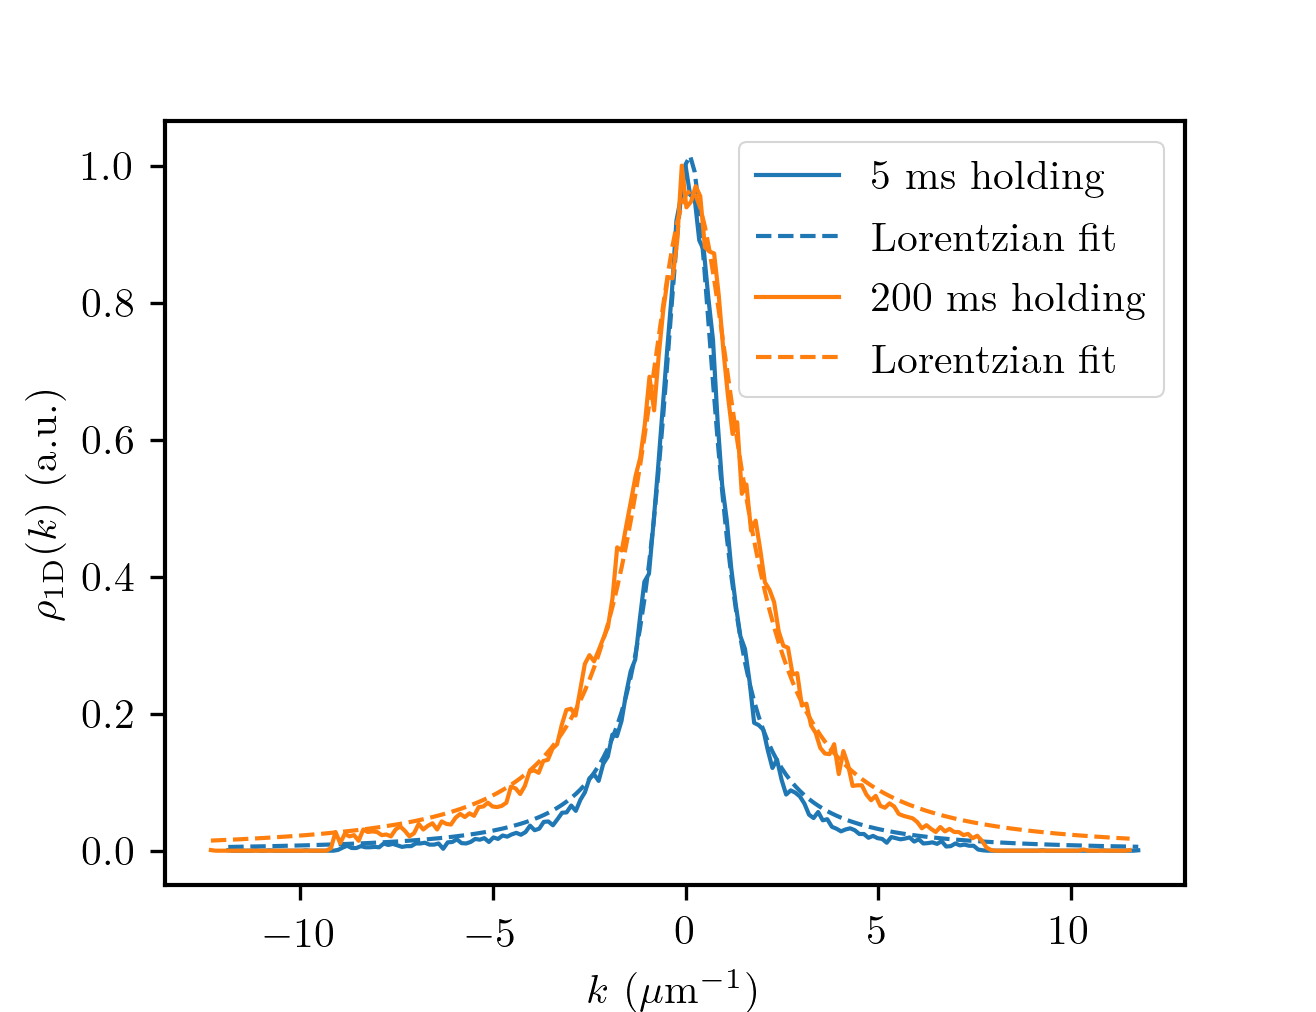
\includegraphics[width=0.8\textwidth]{Fig/Chapter5/1D_temperature_lorentz.png}
    \caption{Normalized 1D momentum distribution $n_{\rm{1D}} (k)$ for lattice holding times $t_{\rm{hold}}=5 \ \rm{ms}$ and $t_{\rm{hold}}=500 \ \rm{ms}$. The Lorentzian fit well matches the data at low $k$. The increase in the width of the distribution signals the increase in temperature induced by the increased holding time in the lattice.}
    \label{fig:1D_temperature}
\end{figure}

\NOTE{a détailler}

\subsection{Interaction parameter}

The other relevant parameter affecting the value of Tan's contact besides temperature is the interaction parameter $\gamma$. It writes:

\begin{equation}
    \gamma = \frac{m g_{1D}}{\hbar^2 \rho_{1D}(0)}
    \label{eq:gamma}
\end{equation}

\noindent and can be calculated from the number of atoms in a tube, itself deduced from the total atom number with the algorithm presented in \NOTE{ref}. Table \ref{tab:gamma_vs_N} shows its mininmum, maximum, and weighted average value over the ensemble of 1D gases for data sets with different atom numbers.


\begin{table}[h!]
\centering
{\rowcolors{2}{white}{MainColor!12}
    \begin{tabular}{c|c|c|c}
        {\color{MainColor} N} &  {\color{MainColor}$\gamma_{\rm{min}}$} & {\color{MainColor}$\gamma_{\rm{max}}$} & {\color{MainColor}$\mean{\gamma}$}  \\
        \hline
        3.10 $\times 10^4$  & 0.259 & 2.17 & 0.416 \\
        1.10 $\times 10^5$ & 0.156 & 1.63 & 0.252 \\
        2.26 $\times 10^5$ & 0.117 & 1.44 & 0.190 \\
    \end{tabular}}
\caption{Variations of the interaction parameter $\gamma$ among the 1D tubes for different total atom numbers.}
\label{tab:gamma_vs_N}
\end{table}

\subsection{Experimental procedure and first extracted values of the Tan's contact}

The procedure to measure Tan's contact for a given data set is as follows:

\begin{itemize}
    \item We prepare the parameters of the experiment to reach the desired values of temperature and atom number. The latter is calibrated via absorption imaging while the former is set roughly by changing the holding time in the lattice and checking that the width of the 1D distribution increases. 
    \item We start by taking $\sim 100$ experimental shots with no gradient to measure the low $k$ distribution from which we can extract the temperature as explained in \ref{sec:1D_temperature}. We do not need to take a large number of shots as the signal is quite high and we do not require a very high signal to noise ratio to obtain the temperature.
    \item We set the gradient to shift the momentum distribution to access the momentum region where the the $\kmf$ tails are supposed to be present as explained in \NOTE{ref}. Usually, the displacement is not too high so that the momentum range overlaps the natural momentum range of the $\He$ detector where no gradient is used, allowing to check that the displaced data matches nicely the non displaced data in the region of the overlap. 
    \item After computing the 1D distribution $n_{\rm{1D}} (k)$ with the method detailed in \ref{sec:1D_calculation_momentum_density}, we plot the quantity $n_{\rm{1D}} (k) \times k^4$. The presence of $\kmf$ tails is signaled by a flat zone that we can fit with a constant function to extract the bare value of the contact $C$ as illustrated on Fig.-\ref{fig:1D_plots}.

    
\end{itemize}  
    
\begin{figure}
    \centering
    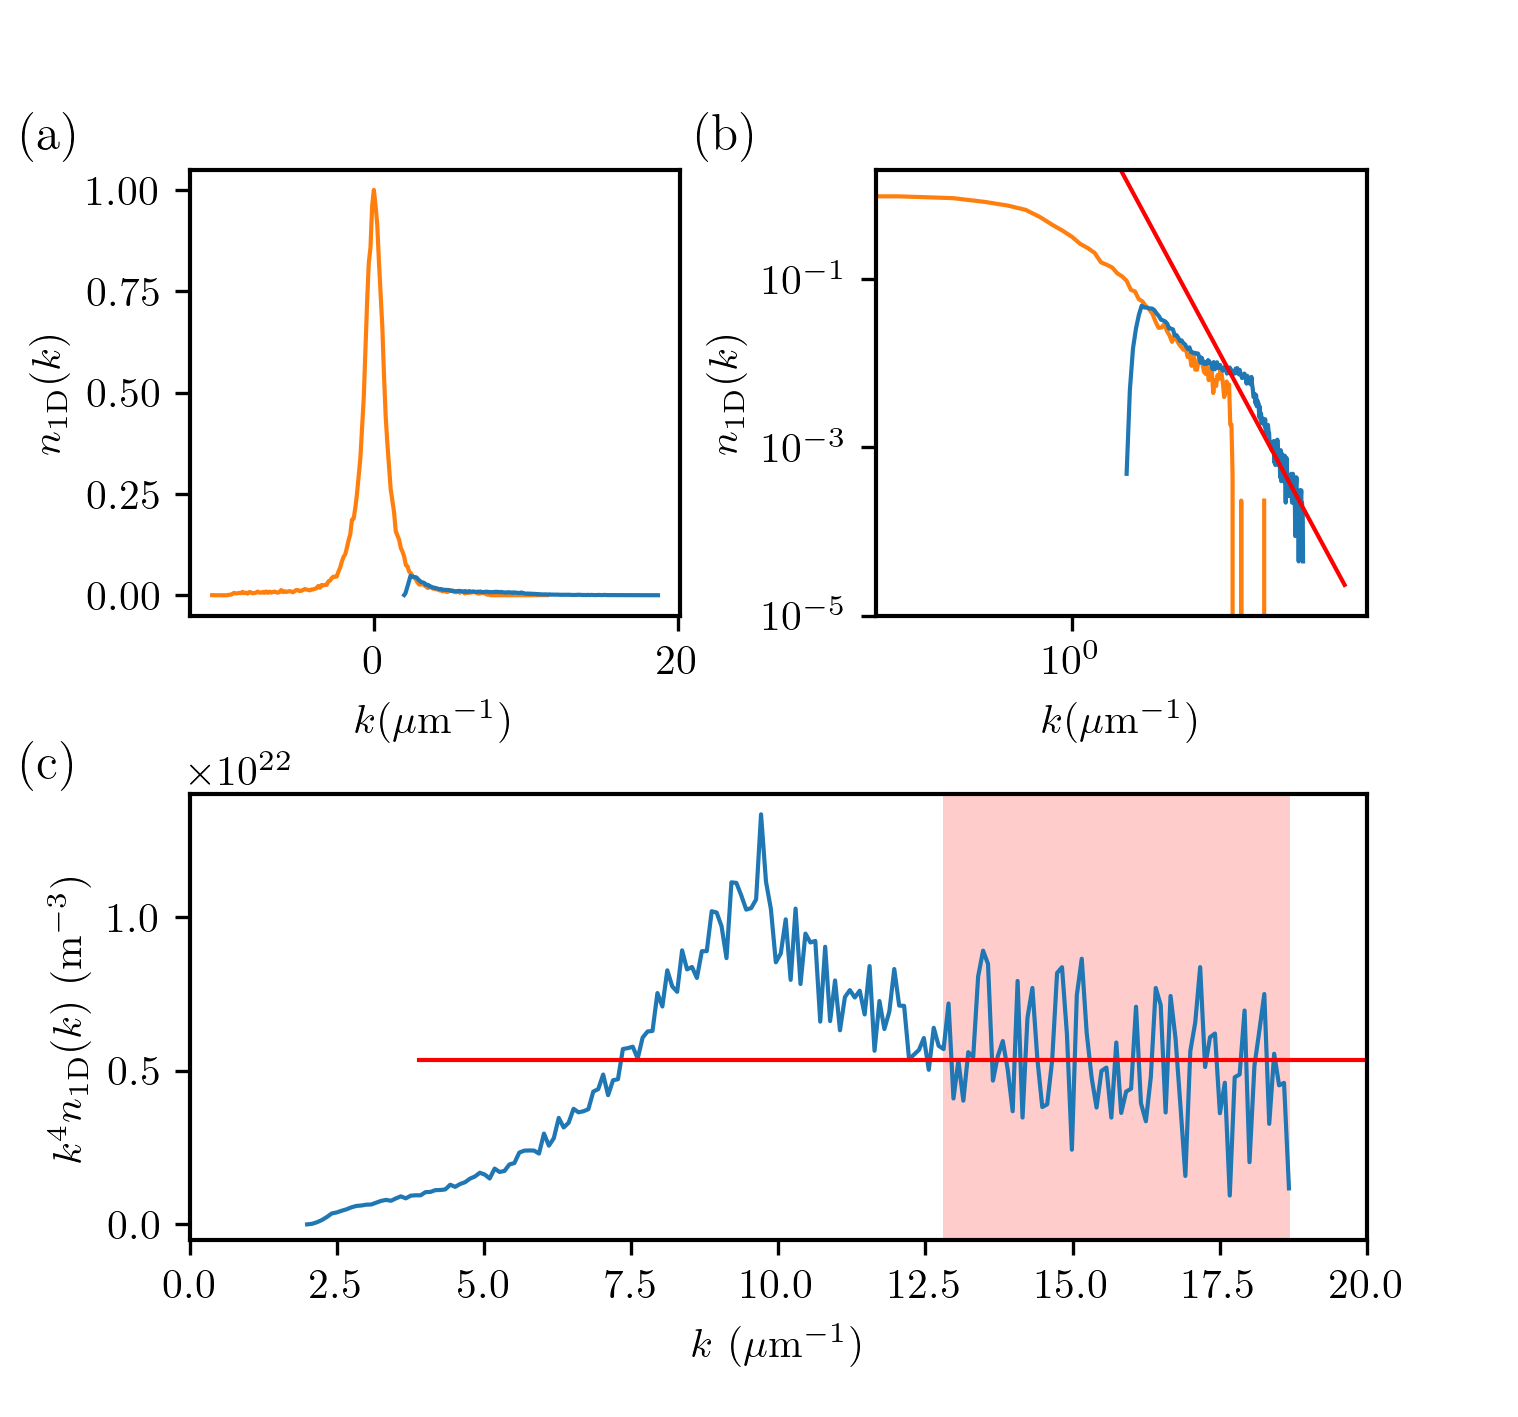
\includegraphics[width=0.95\textwidth]{Fig/Chapter5/1D_plots.png}
    \caption{Plots of $n_{\rm{1D}}$ for $s=26$, $N=3.1(3) \times 10^4$ and $t_{\rm{hold}}=5 \ \rm{ms}$. (a) Linear scale plot of the normalized $n_{\rm{1D}}$ for two momentum ranges. (b) Same data in log scale. The red line indicates a $k^{-4}$ fit. (c) $k^4 n_{\rm{1D}} (k)$ at high momentum. The red shaded area indicates the flat zone of the $\kmf$ tail.}
    \label{fig:1D_plots}
\end{figure}

In order to compare conveniently the experimental data to the theoretical work of \cite{yao2018tan}, we introduce two dimensionless quantities. The first one is the reduced temperature:

\begin{equation}
    \xi_T=-a_{\rm{1D}}/\lambda_T
\end{equation}

\noindent with $a_{\rm{1D}}$ the 1D scattering length and $\lambda_T=\sqrt{2\pi \hbar^2/m k_b T}$. The second one is the reduced the interaction strength:

\begin{equation}
    \xi_{\gamma}=-a_{\rm{ho}}/a_{\rm{1D}}\sqrt{N}
\end{equation}

\noindent with $a_{\rm{ho}}=\sqrt{\hbar/m \omega}$ the harmonic oscillator length. The calculations presented in \cite{yao2018tan} show that 

\begin{equation}
    C= \frac{N^{5/2}}{a_{\rm{ho}}^3} f(\xi_{\gamma},\xi_{T})
\end{equation}

\noindent We can then define a rescaled contact

\begin{equation}
    \tilde{C}=C \frac{a_{\rm{ho}}^3}{N^{5/2}}
\end{equation}

\noindent which depends only on $f(\xi_{\gamma},\xi_{T})$, $\xi_{\gamma}$ and $\xi_{T}$ then being the good parameters to characterize the contact. The ultimate goal of the experiment would then be to characterize the evolution of $f(\xi_{\gamma},\xi_{T})$ and compare it to the predictions of \cite{yao2018tan}. Our quantity of interest will then be the rescaled contact $\tilde{C}$.

\subsubsection{Effect of temperature}

We plot on Fig.-\ref{fig:C_tilde_vs_T} the experimental rescaled contact $\tilde{C}$ as a function of $\xi_T$ for a fixed atom number $N=1.1 \times 10^5$ corresponding to $\xi_{\gamma}=0.113$. The error bars corresponds to the standard deviation over the data points averaged to obtain the value of the contact. \NOTE{terminer avec partie théorique}

\begin{figure}
    \centering
    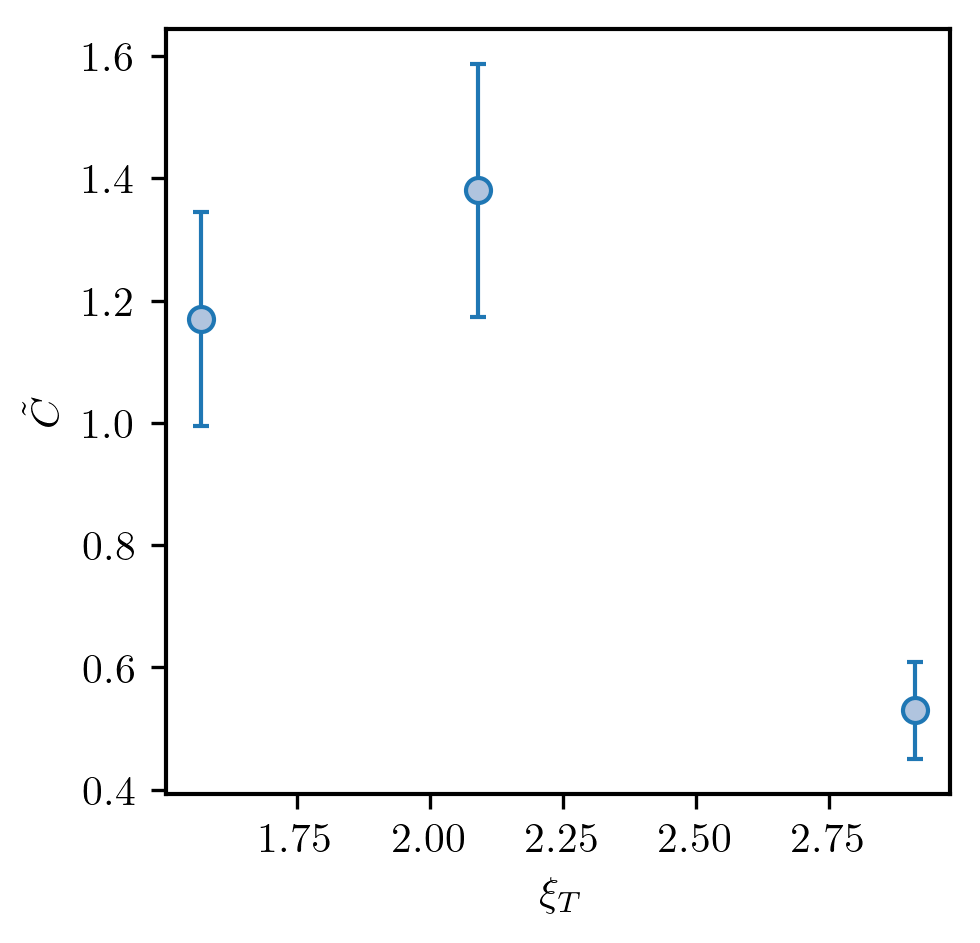
\includegraphics[width=0.6\textwidth]{Fig/Chapter5/C_tilde_vs_T.png}
    \caption{Rescaled contact $\tilde{C}$ as a function $\xi_T$. \NOTE{finir la caption avec partie théorique}}
    \label{fig:C_tilde_vs_T}
\end{figure}

\subsubsection{Effect of the total atom number}

\subsection{Comparison with QMC calculations}

\section{Discussion of the preliminary results}